\section*{CHƯƠNG 2. NỘI DUNG THỰC TẬP}
\setcounter{section}{2}
\setcounter{subsection}{0} %LƯU Ý MỖI LẦN THÊM CHƯƠNG MỚI CẦN THÊM CÂU NÀY ĐỂ RESET THỨ TỰ CỦA SUBSECTON VỀ 1
\setcounter{table}{0} % LƯU Ý SAU MỖI LẦN GỌI BẢNG HAY HÌNH ẢNH PHẢI THÊM CÂU NÀY ĐỂ RESET THỨ TỰ
\setcounter{figure}{0} %% LƯU Ý SAU MỖI LẦN GỌI BẢNG HAY HÌNH ẢNH PHẢI THÊM CÂU NÀY ĐỂ RESET THỨ TỰ
\addcontentsline{toc}{section}{\numberline{}CHƯƠNG 2. NỘI DUNG THỰC TẬP}

Đây là chương em sẽ trình bày về các công việc đã làm được trong thời gian thực tập tại công ty TNHH Pancake Việt Nam.
Em là thực tập sinh ở vị trí lập trình viên phần mềm cho ứng dụng Pancake Chat. Ứng dụng hỗ trợ người dùng quản lý
công việc. Dưới đây là các công cụ mà em được học và sử dụng:

\subsection{Công cụ sử dụng}
\subsubsection{Flutter}
Flutter là framework được chúng em sử dụng để lập trình cho Pancake Chat. Nó là một framework mã nguồn mở phát triển bởi Google, được sử dụng để xây dựng ứng dụng di động, web và desktop đẹp và nhanh chóng. 
Flutter sử dụng ngôn ngữ lập trình Dart, là một ngôn ngữ hiện đại và linh hoạt, giúp tạo ra các ứng dụng chạy mượt mà trên nhiều nền tảng.

\begin{figure}[H]
  \centering
  \includegraphics[width=12cm,height=5.4cm]{Images/flutter_cover.png}
  \caption[Logo Flutter]{\bfseries \fontsize{12pt}{0pt}
  \selectfont Logo Flutter}
  \label{flutter_cover} 
\end{figure}

Một số điểm nổi bật của Flutter được chúng em sử dụng bao gồm:

\begin{itemize}
  \item Giao diện được xây dựng dễ dàng với Widgets, chức năng được tuỳ biến và phát triển với Library.
  \item Tích hợp nhanh chóng: Flutter hỗ trợ tích hợp API của hệ điều hành và bên thứ ba một cách dễ dàng, giúp chúng ta tạo các tính năng phong phú và đa dạng cho ứng dụng của mình
  \item Tương thích đa nền tảng: Với Fluter, mã nguồn cơ sở chỉ cần viết một lần và triển khai ứng dụng của mình trên nhiều nền tảng như Android, iOS, web và desktop mà không cần viết lại mã nguồn
\end{itemize}
\subsubsection{Elixir}
Elixir là một ngôn ngữ lập trình chạy trên môi trường Erlang, được thiết kế để xây dựng các ứng dụng phân tán, 
đáng tin cậy và có hiệu suất cao. Elixir kế thừa rất nhiều tính năng mạnh mẽ từ Erlang, nhưng lại có cú pháp 
và cách viết gần gũi hơn với lập trình viên hiện đại.

Dưới đây là một số điểm quan trọng về Elixir:
\begin{itemize}
  \item Elixir là một ngôn ngữ lập trình hướng hàm, nghĩa là nó tập trung vào việc sử dụng hàm và biểu thức để thực hiện các tính toán
  \item Elixir được xây dựng trên nền tảng Erlang, cho phép bạn xử lý các tác vụ đồng thời và song song một cách hiệu quả
  \item Elixir khuyến khích sử dụng dữ liệu không thay đổi, điều này giúp tránh rất nhiều vấn đề liên quan đến đồng thời và xử lý lỗi
\end{itemize}

\begin{figure}[H]
  \centering
  
\includegraphics[width=12cm,height=4.5cm]{Images/pancake/elixir.png}
  \caption[Logo Elixir]{\bfseries \fontsize{12pt}{0pt}
  \selectfont Logo Elixir}
  \label{firebase_cover} 
\end{figure}


\subsubsection{Firebase Cloud Messaging}

Firebase Cloud Messaging (FCM) là một dịch vụ của nền tảng Firebase của Google, cho phép bạn gửi thông báo và 
tin nhắn đến các ứng dụng di động (Android, iOS) và các thiết bị web (trình duyệt) một cách hiệu quả và đáng tin cậy. 
FCM giúp bạn tương tác và giữ liên lạc với người dùng của ứng dụng của mình thông qua các thông báo thời gian thực.

Đặc điểm của Firebase Cloud Messaging bao gồm:
\begin{itemize} 
  \item Gửi thông báo đa nền tảng
  \item FCM hỗ trợ gửi thông báo thời gian thực (real-time notifications), giúp người dùng nhận được thông báo ngay lập tức khi có sự kiện quan trọng diễn ra trên ứng dụng
  \item Được tích hợp sâu với các sản phẩm và dịch vụ khác của Firebase, như Firebase Authentication, Firebase Cloud Functions
\end{itemize}

\begin{figure}[H]
  \centering
  \includegraphics[width=12cm,height=3cm]{Images/firebase_cover.png}
  \caption[Logo Firebase]{\bfseries \fontsize{12pt}{0pt}
  \selectfont Logo Firebase}
  \label{firebase_cover} 
\end{figure}

\subsection{Nội dung thực tập}
\subsubsection{Yêu cầu công việc}
Các yêu cầu cụ thể ở vị trí thực tập là:
  \begin{itemize}
    \item Tham gia trực tiếp các sản phẩm công ty đang phát triển và các phần mềm hỗ trợ quản lý trong công ty
    \item Ưu tiên có kiến thức Javascript (ReactJS hoặc VueJS) đối với Web và Flutter đối với Mobile
    \item Ham học hỏi, có thể làm việc độc lập
    \item Ưu tiên đã làm việc với API
  \end{itemize}

\subsubsection{Các công việc được giao trong đợt thực tập}
Trong thời gian thực tập em được phân nhiệm vụ xử lý các bug nhỏ trong ứng dụng Pancake Chat:
\begin{itemize}
  \item Xử lý lỗi giao diện app
  \item Thực hiện chức năng "forward file" trong ứng dụng
  \item Sửa các lỗi chức năng nhỏ trong máy Win và MacOS
\end{itemize}

\begin{figure}[H]
  \centering
  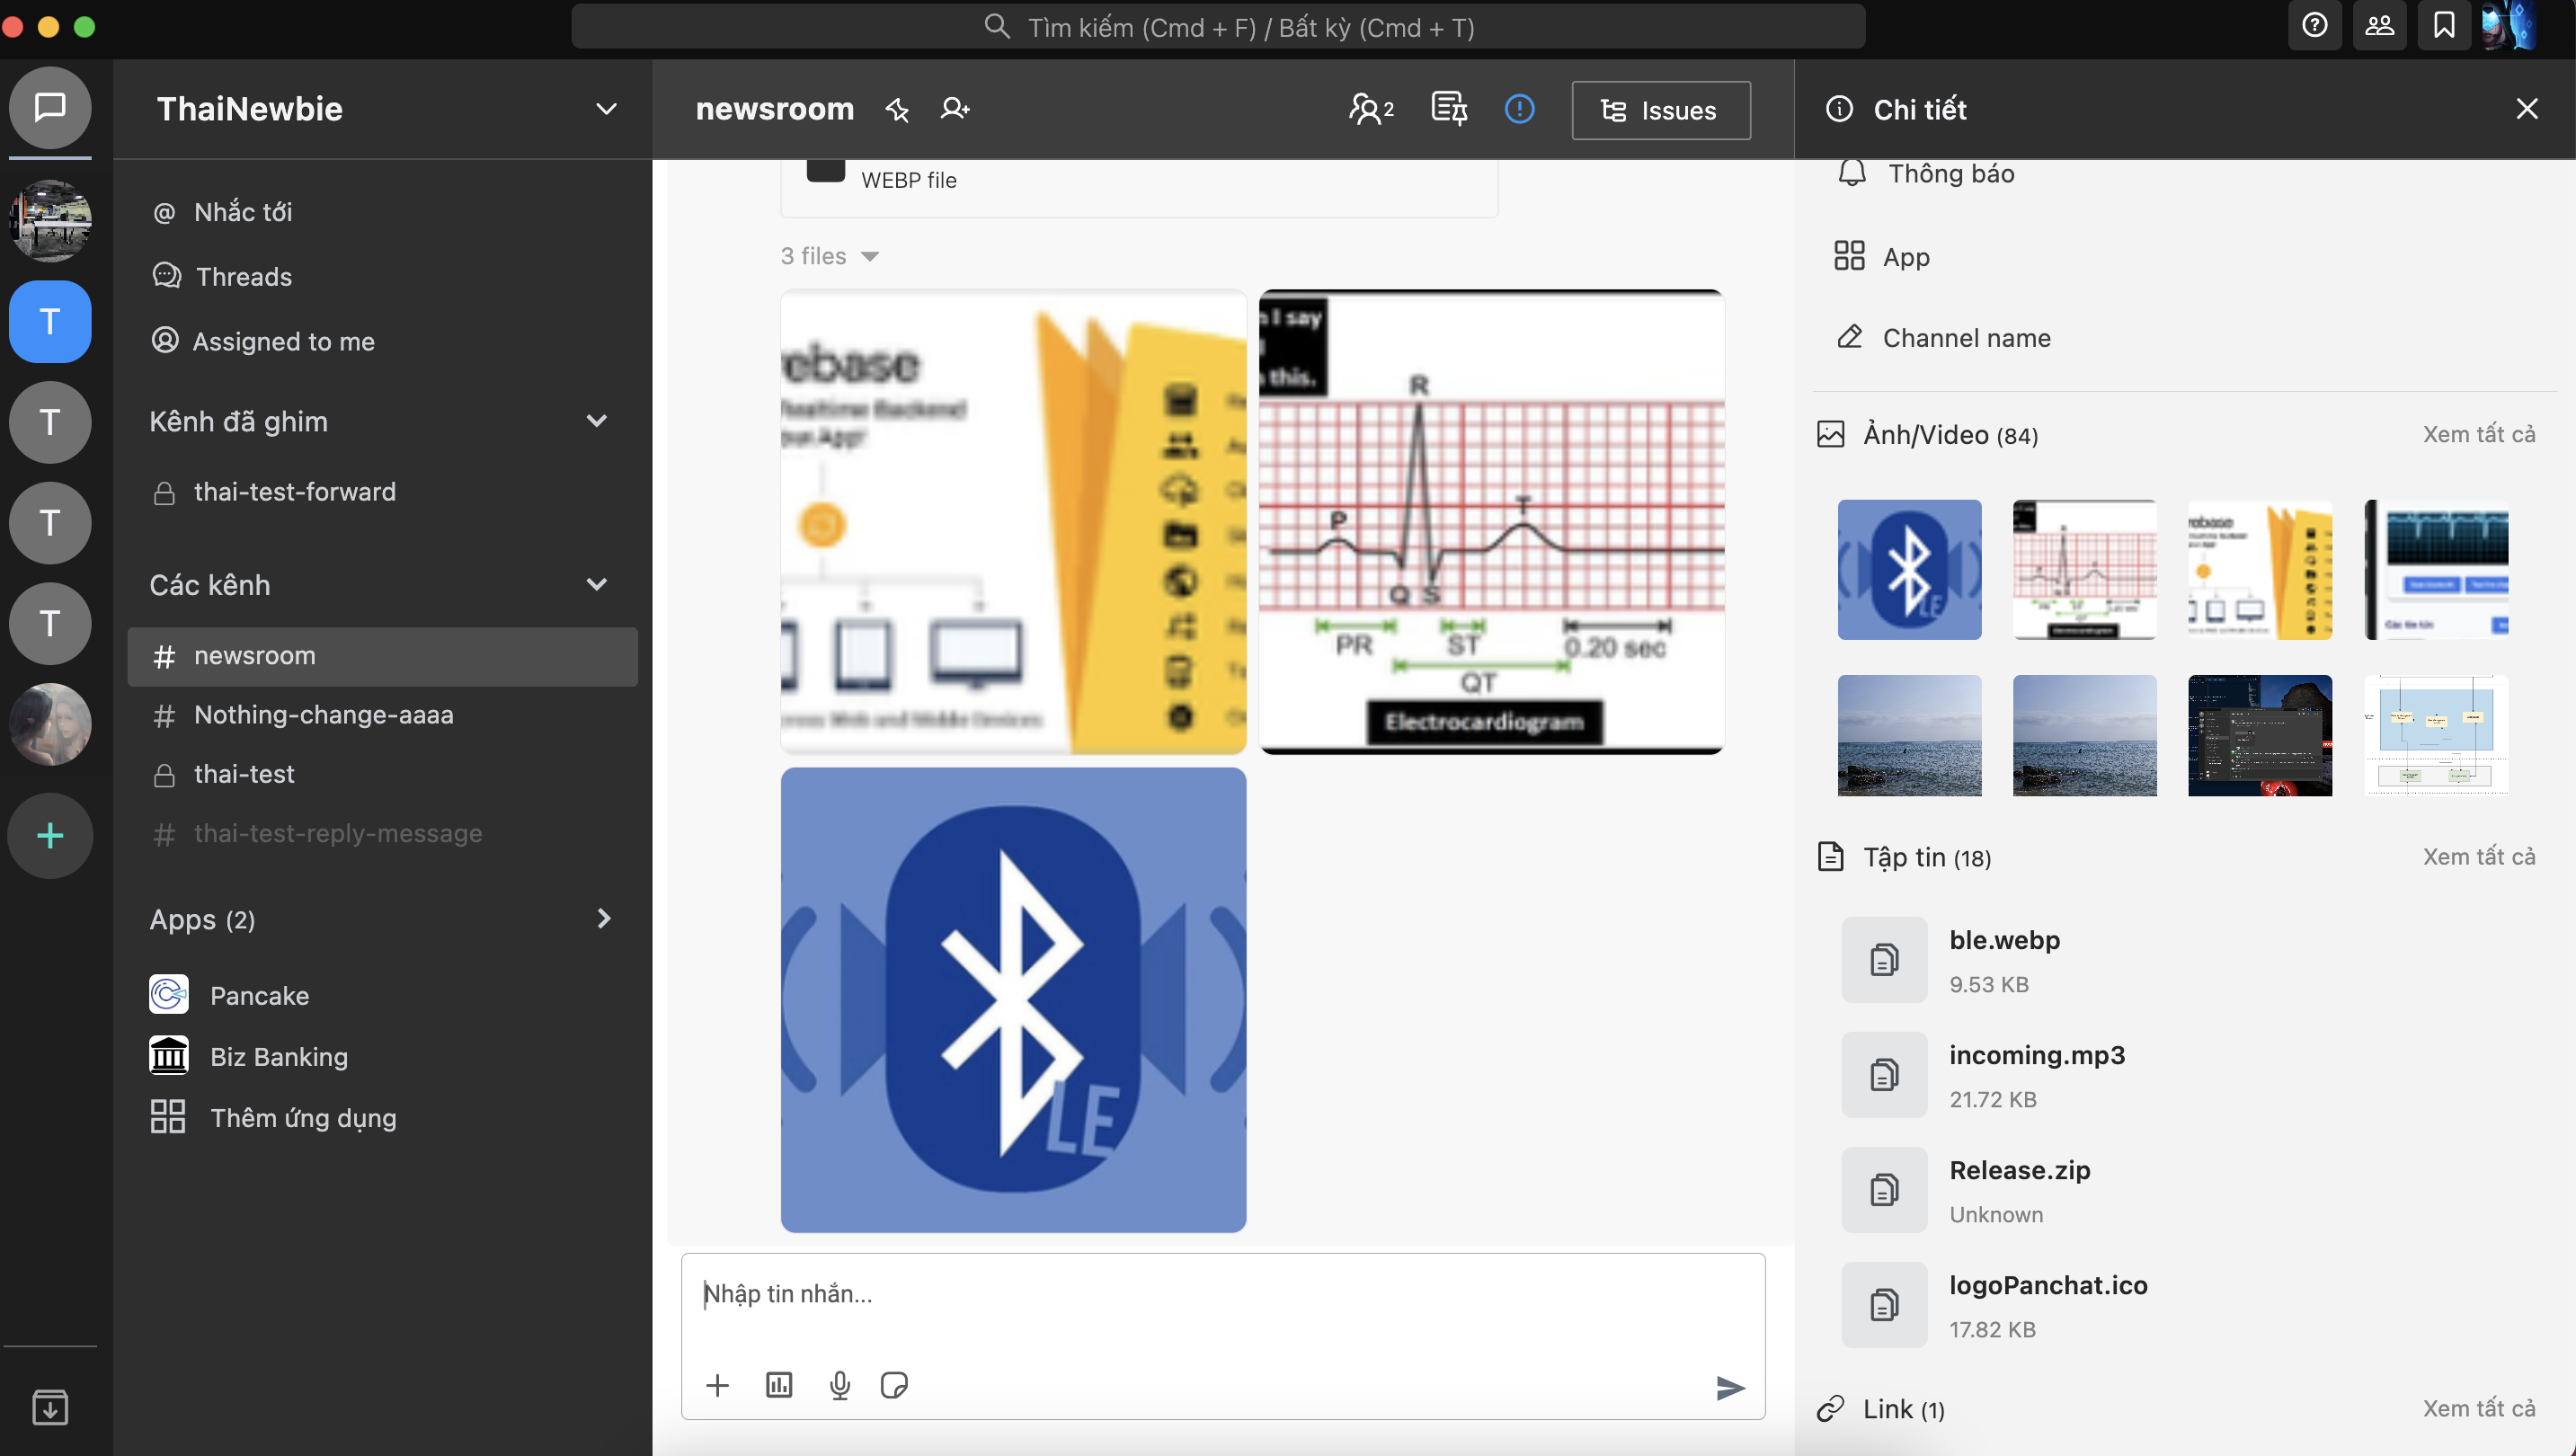
\includegraphics[width=14cm,height=8cm]{Images/pancake/panchat_channel.png}
  \caption[Hình ảnh giao diện channel trong ứng dụng Pancake Chat]{\bfseries \fontsize{12pt}{0pt}
  \selectfont Hình ảnh giao diện channel trong ứng dụng Pancake Chat}
  \label{pancake_chat_channel} 
\end{figure}


\begin{figure}[H]
  \centering
  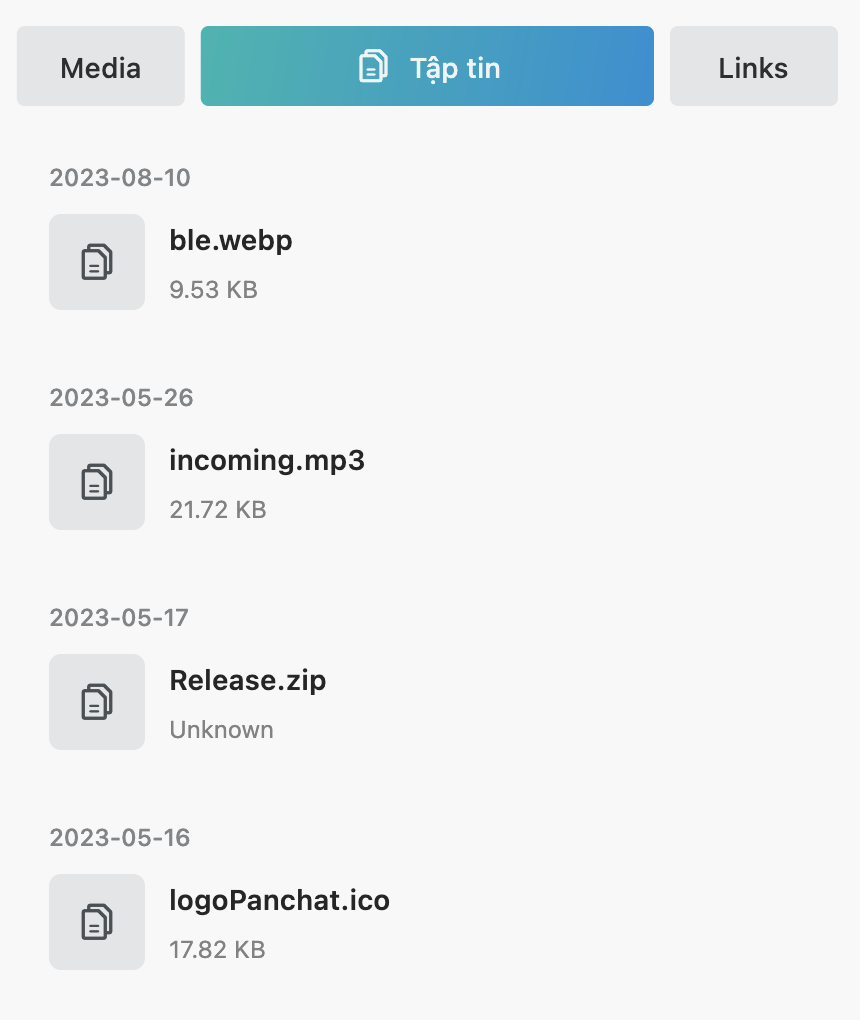
\includegraphics[width=9cm,height=10cm]{Images/pancake/panchat_files.png}
  \caption[Giao diện lưu file trong ứng dụng Pancake Chat]{\bfseries \fontsize{12pt}{0pt}
  \selectfont Giao diện lưu file trong ứng dụng Pancake Chat}
  \label{panchat_files} 
\end{figure}

\begin{figure}[H]
  \centering
  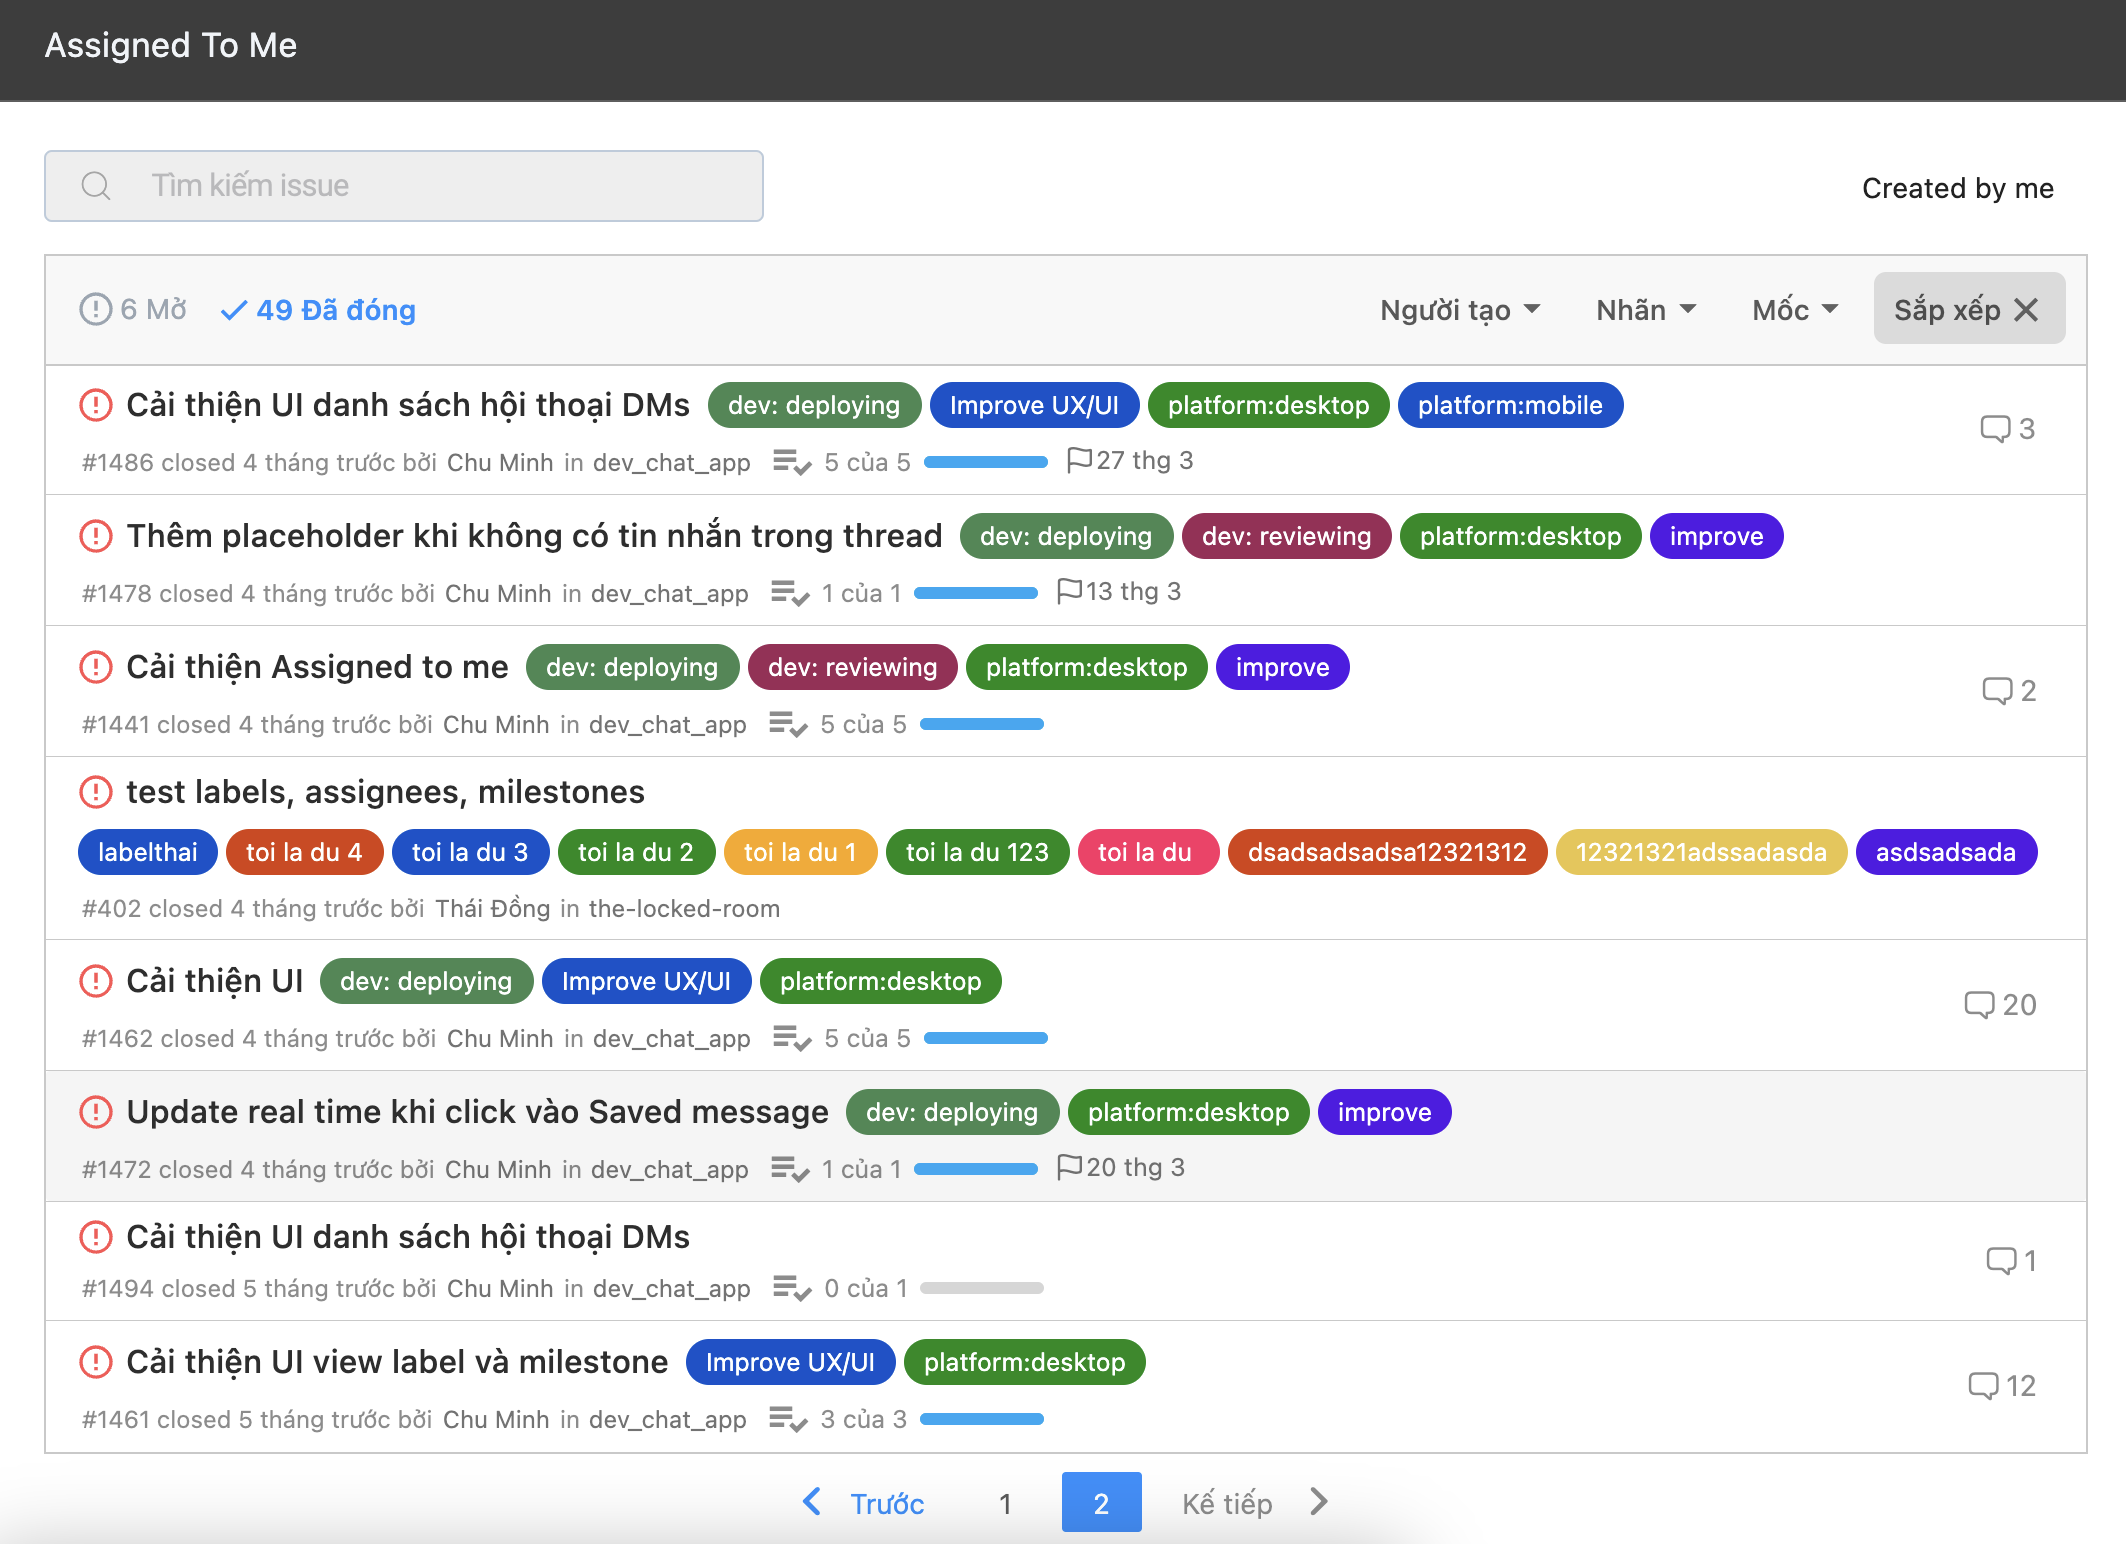
\includegraphics[width=9cm,height=10cm]{Images/pancake/panchat_issue.png}
  \caption[Giao diện phân chia công việc trong ứng dụng Pancake Chat]{\bfseries \fontsize{12pt}{0pt}
  \selectfont Giao diện phân chia công việc trong ứng dụng Pancake Chat}
  \label{panchat_issue} 
\end{figure}

Sau khi hoàn thành được một issue sẽ thực hiện tạo yêu cầu trong một hệ thống quản lý phiên bản để
thấy được sự thay đổi của nội dung trước và sau khi làm. Các yêu cầu sẽ được leader kiểm tra và nếu phù hợp sẽ
được đẩy vào trong nhánh chính, nếu không sẽ được yêu cầu sửa đổi để phù hợp với cả nhóm.

\subsection{Kết luận chương}
Trong chương này, em đã trình bày về các công cụ mà em được sử dụng và các công việc được giao trong thời gian
thực tập.
\newpage